\chapter{Quantum mechanics on a computer}

This chapter comprises a summary of some of the methods used by cold atom physicists to compute numerical results pertaining to cold atom systems. Many a problem in quantum mechanics is not analytically solvable, especially when the real world of experimental physics rears its ugly head, violating theorists' assumptions of simplicitly left and right. In particular, atomic physics experiments are time-dependent, with each run of an experiment generally proceeding in stages. Lasers may turn on and off, magnetic fields may vary in magnitude and direction, \textsc{rf} pulses may be chirped [CITE LISA?] to reliably induce particular atomic transitions. Much of the numerical calculations performed by researchers in cold atom physics groups such as ours are accordingly of the time-dependent variety, and are fairly literal simulations of specific experiments that may be carried out in the lab.

\section{From the abstract to the concrete: neglect, discretisation and representation}

To numerically simulate a quantum mechanical system, one must evolve a state vector in time according to the Schr\"odinger equation:
\begin{align}\label{eq:schrodinger_equation}
i\hbar\dv{t}\ket{\psi(t)} = \hat H (t) \ket{\psi(t)}
\end{align}
To do this on a computer, one must first decide which degrees of freedom are to be simulated. We necessarily neglect many degrees of freedom as a matter of course; which ones can be neglected is warranted by the specific situation and we do it so often we barely notice. For example, simulating a single component Bose--Einstein condensate entails neglecting the internal degrees of freedom of the atoms---as well as reducing the atom-light interaction to a simple potential such as an optical dipole trap or magnetic dipole interaction (neglecting the quantum degrees of freedom in the electromagnetic field). We may ignore one or more spatial degrees of freedom as well, say, if we are simulating an experiment in which the condensate is confined to two dimensions by way of a tight trapping potential in one direction [CITE AN EXAMPLE]. Or, when simulating laser cooling [SEE SECTION TODO], we may care very much about the electronic state of the atom, but treat its motional state classically. In these cases we are essentially imposing the assumption that the system will only occupy one state with respect to those degrees of freedom ignored (the condensate will remain in lowest excitation level in the direction of the tight trap, the atoms will remain in one specific Zeeman sublevel), or we are assuming those degrees of freedom can be treated classically (the electromagnetic field is well described by classical electromagnetism, the atoms' motional state is described well by Newtonian mechanics). Which degrees of freedom can be neglected and which cannot requires knowledge of the situation at hand, often informed by best-practices of the research community in question and ultimately justified by experiment.\footnote{A classic example in the cold atom community of neglected degrees of freedom leading to \emph{disagreement} with experiment is the discovery of polarisation gradient cooling (\textsc{PGC}) [CITE THE LIGHT SHEET EXPERIMENT], the explanation for which requires consideration of Zeeman sublevels of the atoms. The experiment that discovered \textsc{PGC} was designed to measure the effect of Doppler cooling, which does not involve Zeeman sublevels, and it was not until afterwards that theorists determined [CITE DALIBARD ETC] that transitions between Zeeman sublevels cannot be neglected and indeed are crucial in explaining the lower than predicted temperatures observed.}

Once the degrees of freedom are known, one must decide on a basis in which to represent them concretely. The basis often cannot be complete, since for many degrees of freedom this would require an infinite number of basis states---for example the electronic state of an atom contains a countably infinite number of states, and a spatial wavefunction in free space has an uncountable number of states (one for each position in R3 [TODO BLACKBOARD BOLD]). For the internal state of an atom, therefore, we restrict ourselves to only the states we expect can become non-negligibly occupied, given the initial conditions and transitions involved. For example, at low temperature we can expect atoms to be almost completely in their electronic ground states, since energy gaps between ground and excited states are large compared to the atoms' thermal energy.\footnote{The D-line of rubidium 87 has an energy gap of [TODO], requiring a temperature of [TODO] or higher in order for the Boltzmann factor $e^{\frac{\upDelta E}{kT}}$ describing the excited state population to be greater than $1\E{-6}$.}. We need only include the small number of excited states that might become occupied as a result of optical transitions present in the situation being simulated. This can still be a large number of states if one is studying Rydberg atoms [CITE] or using ultrafast (and therefore broad-band) laser pulses, but is otherwise fairly small. For example, including both the D1 and D2 lines of Rubidium 87, with all hyperfine levels and Zeeman sublevels gives 32 states (see section [TODO]).

For spatial degrees of freedom, one can either discretise space on a grid, or use a set of orthogonal basis functions\footnote{Strictly speaking, these can be the same thing---discretising space on a grid is declaring one's basis functions to be a set of functions, one for each gridpoint, each of which is zero at all gridpoints .}.


Once the degrees of freedom and basis vectors have been chosen, the state vector is then represented on a computer as an array of complex numbers, giving the coefficients of each basis vector required to represent a particular state vector. Matrix elements of the Hamiltonian in the same basis must be calculated, and the Schr\"odinger equation can then be written:
\begin{align}
i\hbar\dv{t}\braket n{\psi(t)} = \sum_m\matrixel n {\hat H(t)} m \braket m {\psi(t)},
\end{align}
or in standard matrix/vector notation (without Dirac notation):
\begin{align}
i\hbar\dv{t}\psi_n(t) = \sum_m H_{nm}(t) \psi_m(t),
\end{align}
where $\psi_n(t) = \braket n{\psi(t)}$ and $H_{nm}(t) = \matrixel n {\hat H(t)} m$.
This is now something very concrete that can be typed into a computer. Programming languages generally don't know about Dirac kets and operators, and so everything that is to be computed must be translated into matrices and vectors in specific bases. This may seem so obvious as to not be worth mentioning, but was nonetheless a stumbling block in my own experience of getting to grips with quantum mechanics. Once realising that every operator has a matrix representation in some basis, at least in principle, and that every ket is just a list of vector components in some basis, similarly at least in principle, expressions dense in bras and kets become much more concrete as the reader has a feel for exactly how they would type it into a computer. Without this realisation, doing quantum mechanics on paper can seem like an exercise in abstract mumbo-jumbo.

\section{Solution to the Schr\"odinger equation by direct exponentiation}
As an example of something seemingly abstract being more concrete than first appearances, it is sometimes said that the `formal' solution to the Schr\"odinger equation \eqref{eq:schrodinger_equation} is:
\begin{align}\label{eq:formal_solution}
\ket{\psi(t_f)} = e^{-\frac i \hbar \int_t^{t_f} \hat H(t^\prime)\,\dd t^\prime}\ket{\psi(t)}.
\end{align}
Saying that this is the `formal' solution rather than just `the solution' is presumably intended to emphasise that the arithmetic operations involved in \eqref{eq:formal_solution} might not make immediate sense for the types of mathematical objects they are operating on, and that we have to be careful in defining the operations such that they produce a result that is not only sensible, but also the solution to the Schr\"odinger equation. If both $\hat H(t)$ and $\ket{\psi(t)}$ were single-valued functions of time rather than an operator valued function of time (the values at different times of which don't necessarily commute) and a vector valued function of time, then we would have no problem. However, \eqref{eq:formal_solution} as written with operators and vectors is ambiguous, and we need to elaborate on it in order to ensure it is correct. I will come back to this after considering a simpler case.

If the Hamiltonian is time-independent, then \eqref{eq:formal_solution} reduces to
\begin{align}
\ket{\psi(t_f)} = e^{-\frac i \hbar (t_f - t)\hat H}\ket{\psi(t)}.
\end{align}
Given the matrix representation $H$ of $\hat H$ and vector representation $\psi(t)$ of $\ket{\psi(t)}$ in a particular basis, this can now be directly typed into a computer as the matrix multiplication:
\begin{align}
\psi(t_f) = U(t, t_f)\psi(t),
\end{align}
where
\begin{align}
U(t, t_f) = e^{-\frac i \hbar (t_f - t) H}
\end{align}
is the unitary evolution operator for time evolution from the initial time $t$ to time $t_f$, and is computed using a matrix exponential of $-\frac i \hbar (t_f - t) H$. Exponentiation of matrices is defined via the Taylor series of the exponential,
\begin{align}
e^A = \sum_{n=0}^\infty \frac{A^n}{n!},
\end{align}
which reduces exponentiation to the known operations of matrix multiplication and addition. However, any linear algebra programming library worth the bytes it occupies will have a matrix exponentiation function that should be used instead, as there are other methods of computing matrix exponentials that are more computationally efficient and numerically stable, such as the Pad\'e approximant [CITE].

\subsection{Matrix exponentiation by diagonalisation}
Regardless of which method is used, matrix exponentiation is computationally expensive. It can be sped up however if a diagonalisation of $H$ is known, since if
\begin{align}
H = UDU^\dagger,
\end{align}
where $D$ is a diagonal matrix and U is a unitary matrix\footnote{Note that the diagonals of $D$ are the eigenvalues of $H$, and the columns of $U$ are its eigenvectors.}, then
\begin{align}
e^{-\frac i \hbar (t_f - t) H} = U e^{-\frac i \hbar (t_f - t)D} U^\dagger.
\end{align}
This is simple to evaluate because the exponentiation of a diagonal matrix can be performed by exponentiating each diagonal matrix element individually\footnote{The reason for this is clear from the Taylor series definition of matrix exponentiation, since matrix multiplication and addition can both be performed elementwise for diagonal matrices.}

Even if a diagonalisation of $H$ is not analytically known, numerically diagonalising $H$ (using a linear algebra library function or otherwise) can form the basis for writing your own matrix exponentiation function, if needed. I found this necessary for efficiently exponentiating an array of matrices in Python, since the \texttt{scipy} and \texttt{numpy} scientific and numeric libraries at the present time lack matrix exponentiation functions that can act on arrays. Writing a \texttt{for} loop in an interpreted language such as Python to exponentiate the matrices individually in many cases is unacceptably slow, so for these cases\footnote{Such as simulating the internal state of a large number of atoms, or evolving a spinor Bose--Einstein condensate by exponentiating the Zeeman Hamiltonian with a spatially varying magnetic field.} I use a function such as the below:

\python{code_listings/expm_example.py}

This concludes all I have to say for the moment on evolving systems with time-independent Hamiltonians using direct exponentiation. Sections [TODO - refer to operator product sections] will say a bit more about how to \emph{approximately} exponentiate certain Hamiltonians, which is sometimes useful. In addition, it turns out that the time-dependent case can be reduced to the repeated application of evolution with time-independent Hamiltonians over small timesteps, as we will see in the next section.

\subsection{Time-ordered exponentials and time-ordered products}


As mentioned, the solution \eqref{eq:formal_solution} is not the whole picture. It can only be taken at face value if the Hamiltonian at each moment in time commutes with itself at all other times [CITE SOMETHING]. In this case, once represented in a specific basis, the solution to the Schr\"odinger equation is again the matrix multiplication
\begin{align}
\psi(t_f) = U(t, t_f)\psi(t),
\end{align}
with
\begin{align}
U(t, t_f) = e^{-\frac i \hbar \int_t^{t_f} H(t^\prime)\,\dd t^\prime}.
\end{align}
Since matrix addition can be performed elementwise, so can the integral in the exponent, yielding a matrix which once exponentiated will give the evolution operator $U(t, t + \upDelta t)$ for the solution to the Schr\"odinger equation. If the Hamiltonian at each moment in time does not commute with itself at all other times, however, then the unitary evolution operator for the solution to the Schr\"odinger equation is instead given by the following \emph{time-ordered exponential} [CITE]:
\begin{align}\label{eq:time_ordered_exponential}
U(t, t_f) = \mathcal{T}\left\{e^{-\frac i \hbar \int_t^{t_f} H(t^\prime)\,\dd t^\prime}\right\}.
\end{align}

In this expression, $\mathcal{T}$ denotes the \emph{time-ordering operator}. The time ordering operator reorders terms within products that contain a time parameter (for us, the time parameter is the argument of the matrix $H$), such that the value of the time parameter is smallest on the rightmost term, largest on the leftmost term, and monotonically increasing right-to-left in between. For example:
\begin{align}
\mathcal{T}\left\{H(4)H(1)H(2)H(5)H(3)\right\} = H(5)H(4)H(3)H(2)H(1).
\end{align}

Despite appearances, this time-ordered exponential is perfectly concretely defined via the definitions of all the operations involved that we have described so far, and can---with some effort---be typed into a computer and evaluated directly. Even though this is not how I evaluate time-ordered exponentials in my simulations of atomic systems, I'll quickly elaborate on this just to emphasise the concreteness of all these operations.

``What products is $\mathcal{T}$ reordering?" you might ask, as \eqref{eq:time_ordered_exponential} doesn't appear to contain any products of $H(t)$. On the contrary, it does, since exponentiation is defined by its Taylor series, and so
\begin{align}
U(t, t_f) &= 1 + \mathcal{T}\left\{\sum_{n=1}^\infty \frac1 {n!}\left[ -\frac i \hbar \int_t^{t_f} H(t^\prime)\,\dd t^\prime\right]^n\right\}\\
&= 1 + \sum_{n=1}^\infty \frac{(-i)^n} {n!\hbar^n}\mathcal{T}\left\{\left[\int_t^{t_f} H(t^\prime)\,\dd t^\prime\right]^n\right\}\,.
\end{align}
Each term in this series contains the $n^\up{th}$ power (and hence a product) of an integral of $H(t)$. The time ordering operator doesn't allow us to evaluate each term by computing the matrix integral once and then raising it to a power---to do so would violate time-ordering since each integral involves evaluating $H(t)$ at all times. Instead we have to write each product of integrals as the integral of a product:
\begin{align}
U(t, t_f)
&= 1 + \sum_{n=1}^\infty \frac{(-i)^n} {n!\hbar^n}\int_t^{t_f}\cdots\int_t^{t_f} \mathcal{T}\left\{H(t_1^\prime)\cdots H(t_n^\prime)\right\}\,\dd t_1^\prime\cdots\dd t_n^\prime\,,
\end{align}
from which we can see exactly which product of matrices the time ordering operator is acting on.

Now we are close to seeing one might evaluate $U(t, t_f)$ numerically by summing each term in the Taylor series up to some order set by the required accuracy. For the $n^{\up{th}}$ term, one needs to evaluate an $n$-dimensional integral over $n$ time coordinates, with each coordinate having the same limits of integration. This can be computed in the usual way an integral is numerically computed\footnote{By sampling the integrand on a uniform grid, using a quadrature method, or Monte-Carlo integration [CITE], which is widely used for high dimensional integrals such as these.}, with the minor change that each time the integrand is evaluated, the terms within it must be re-ordered to respect the required time-ordering. Alternatively, the integration region can be restricted to the region in which the terms are already time-ordered, and then the total integral inferred by symmetry, which gives:
\begin{align}
U(t, t_f)
&= 1+\sum_{n=1}^\infty \left(-\frac i \hbar\right)^n\int_t^{t_f}\cdots\int_t^{t_{n-1}^\prime} H(t_1^\prime)\cdots H(t_n^\prime)\,\dd t_1^\prime\cdots\dd t_n^\prime\,.
\end{align}

This is now a perfectly concrete expression, with each term comprising an integral over an $n$-simplex\footnote{A simplex is the generalisation of a triangle to higher dimensions, i.e a 3-simplex is a tetrahedron.} of a product of $n$ matrices.

This expression for the unitary evolution operator is called the Dyson series [CITE]. It is not generally used in cold atom physics; I certainly have never evaluated it. However it does see use in high energy physics [CITE] for computing transition amplitudes between incoming and outgoing waves in scattering problems (in which $U$ is called the $S$-matrix). In these problems, $H$ is an interaction Hamiltonian containing terms for all particle interactions being considered. Accordingly, the integrand for the $n^\up{th}$ term, being a product of $n$ copies of $H$ at different times, contains one term for each possible sequence of $n$ particle interactions.
The integral itself can be considered a sum of transition amplitudes over all possible times that each interaction could have occurred. Indeed, each term corresponds to a Feynman diagram with $n$ nodes [CITE].

The Dyson series isn't really suited to the problems we face in cold atom physics. For one, the series must be truncated at some point, and the result won't be a $U$ that is actually unitary.\footnote{Although unitarity is not often a strict requirement - we also frequently solve [EQREF TDSE] directly with fourth order Runge--Kutta, which is also not unitary.}. Also, we are usually interested in the intermediate states, not just the final state of a system as in a scattering problem.

In any case, typically when solving the Schr\"odinger equation by exponentiation we use the following, alternate expression for a time-ordered exponential:
\begin{align}
U(t, t_f) &= \mathcal{T}\left\{e^{-\frac i \hbar \int_t^{t_f} H(t^\prime)\,\dd t^\prime}\right\}\\
 &= \lim_{N\rightarrow\infty}\mathcal{T}
 \left\{\prod_{i=0}^N e^{-\frac i \hbar  H(t_i)\upDelta t}\right\},
\end{align}

where $\upDelta t = (t - t_f)/N$ and $t_i = t + i\upDelta t$. You can convince yourself that [EQREF INTEGRAL DEFINITION] is equivalent to this by replacing the integral in the exponent with a sum---as per the Riemann definition of an integral---and expanding the exponential according to its Taylor series. Expanding each exponential in [EQREF PRODUCT DEFINITION] as a Taylor Series and collecting terms with the same number of copies of $H$ then reveals that the two Taylor series are identical.

In any case, [EQREF PRODUCT DEFINITION] paints an intuitive picture of solving the Schr\"odinger equation: one evolves the initial state vector in time by evolving it according to constant Hamiltonians repeatedly over small time intervals. This has the desirable property that all intermediate state vectors are computed at the intermediate steps, meaning one can study the dynamics of the system and not just obtain the final state. This is of course useful for comparison with experiments, plenty of which involve time-dependent data acquisition and not just post-mortem analysis of some evolution.

Numerically, we can't actually take $N\rightarrow\infty$, or equivalently $\upDelta t \rightarrow 0$, and so we instead choose a $\upDelta t$ smaller than the timescale of any time-dependence of $H$, and step through time using [EQREF].

Thus the case of a time-dependent Hamiltonian reduces to repeated application of the solution [EQREF] for a time-independent Hamiltonian. Furthermore, if the Hamiltonian is analytically diagonalisable at each moment in time, each of these steps can be taken with the diagonalisation method of matrix exponentiation. If it is not, and the system is small, then resorting to numerical diagonalisation may be acceptable. Otherwise, if the Hamiltonian can be decomposed into a \emph{sum} of terms which are individually diagonalisable, the split-step method can be used (see sec [SECREF]). Failing that, a general purpose integration method such as fourth-order Runge-Kutta may have to be resorted to.\footnote{Though if I admit it, \textsc{rkr4} is usually what I reach for first.} I will elaborate on these comments with examples in the following sections.

\begin{itemize}

\item {absorbing boundary conditions, reflective boundary conditions, periodic boundary conditions}

\end{itemize}

\section{Continuous degrees of freedom}
The single-particle, non-relativistic, scalar Schr\"odinger wave equation, as distinct from the general Schr\"odinger equation [EQREF], is:

[EQUATION].

As mentioned in [SECREF], the equation for the single-particle wavefunction of an atom in a single-component Bose--Einstein condensate is the Gross--Pitaevskii equation

[EQUATION],

where $\psi(\vec r) = \sqrt{N}\braket{\vec r}{\psi}$ is the single-particle wavefunction scaled by the square root number of atoms $N$.

Both these equations are partial differential equations involving both spatial and temporal derivatives. But in quantum mechanics all state vectors can be mapped to column vectors and all operators to matrices. Spatial wavefunctions are no exception to the former and differential operators such as $\grad^2$ are no exception to the latter. So what do these vectors and operators look like? That depends on whether we choose to discretise space on a grid, or use a functional basis (and on which functional basis we choose). As we'll see below, however, spatial discretisation is actually just a particular choice of functional basis, namely the Fourier basis.

\subsection{Spatial discretisation}
Imagine a two dimensional spatial region within which we are solving the single-component Gross--Pitaevskii equation, evolving an initial condensate wavefunction in time. Having specified which degrees of freedom we want to simulate (two continuous degrees of freedom, one for each spatial dimension), the next step according to the method outlined in [SECREF ABOVE] is to choose a basis in which to represent this state vector.

Lets say we discretise space in an equally-spaced $5\times 5$ rectangular grid,\footnote{For the sake of example---$256\times256$ is a more realistic minimum.} with spacing $\upDelta x$, and only represent the wavefunction at those $25$ points in space. The state vector can then be represented by a list of $25$ complex numbers, each taken to be the wavefunction's value at the spatial position corresponding to one gridpoint. This $25$-vector is now a concrete representation of our state vector.

[FIGURE SHOWING UNWRAPPING OF 2D REGION INTO COLUMN VECTOR. PERHAPS 2D REGION IS CONTINUOUS WITH A GRID SUPERIMPOSED ON IT, AND LINES JOIN EACH GRIDPOINT TO THE VECTOR AT RIGHT]

But at what point did we choose a basis just now---what are the basis vectors? This just looks like discretising space at a certain resolution, rather than the formal process of choosing a basis and projecting the state vector and operators onto each basis vector, as outlined in [SECREF ABOVE]. Assuming what we've done is equivalent to choosing a basis, that basis has a finite number ($25$) of basis vectors, which means it cannot be complete, since state vectors we're approximately representing with it require an infinite number of complex numbers to be described exactly.\footnote{One for each position within the two dimensional space we're representing.} So what do the basis functions look like, and what state vectors have we implicitly excluded from simulation by choosing a basis that is incomplete?

As a sidenote, spatial wavefunctions are often described as the representation of wavefuctions in the ``spatial basis"---a basis in which the basis vectors $\{\ket{\vec r}\}$ are Dirac-deltas centred on each point in space [CITE DIRAC'S BOOK MAYBE]. The wavefunction $\psi(\vec r)$ is then simply a coefficient saying how much of the basis vector $\ket{\vec r}$ (the spatial representation of which is a Dirac delta centred on the position $\vec r$) to include in the overall state vector. What we have \emph{not} done is chosen a subset of these Dirac delta basis functions\footnote{Strictly, distribtuions, not functions, but ``basis distributions" just doesn't have the right ring to it.} as our basis. This would be very strange---our representation of the wavefunction would allow it to have a value at one gridpoint, and at the next gridpoint, but not in between. Spatially separated Dirac deltas do not spatially overlap at all; the matrix elements of the kinetic energy operator:
\begin{align}
K_{ij} = \int \delta(\vec r - \vec r_i)\left(-\frac{\hbar^2}{2m}\grad^2\right)\delta(\vec r - \vec r_j)\,\dd \vec r
\end{align}
would all be zero for $i\neq j$, disallowing any flow of amplitude from one point in space to another by virtue of it not being able to pass through the intervening points. Neither have we chosen a set of two-dimenstional boxcar functions centred on each gridpoint with width $\upDelta x$ in each direction. These cover all space in between gridpoints, but are no good because they are not twice differentiable everywhere, and hence the kinetic energy operator's matrix elements cannot be evaluated. No, neither of these bases will do. To interpret our spatial grid as a basis, we need a set of functions [$FUNC_{ij}(r)$] (where $i$ and $j$ are the indices of the gridpoints in the $x$ and $y$ directions respectively) that have unit norm, are nonzero only at one gridpoint and are zero at all others, and are twice differentiable everywhere in our spatial region. Infinite choices present themselves to us, differing only in their incompleteness---the choice of which state vectors they will and won't be able to represent. A sensible choice is that we want to be able to represent the state vectors whose wavefunctions do not change much between adjacent gridpoints, and we are happy for the necessary incompleteness of our basis to exclude wavefunctions with any sort of structure in between gridpoints.

\subsubsection{The discrete Fourier transform to the rescue}

It turns out that discretising space in this way is indeed equivalent to choosing an entirely sensible basis. This is made clearer by thinking in terms of what we have done in Fourier space, which I'll quickly go through now.

Analytically, state vectors in Hilbert spaces with spatial degrees of freedom such as this are often represented in the spatial basis $\ket{\vec r}$. This basis has one basis vector for each point in space (and hence has an infinite number of basis vectors), each of which is a Dirac delta. We then call $\psi(\vec r)$ the \emph{wavefunction} corresponding to the state vector. \footnote{Dirac introduced this distinction when he invented bra-ket notation, that the state-vector's coefficients in a continuous basis can be written as a function of a continuous variable and called a ``wavefunction"}

If the state vector is known in some basis $\ket{n}$, then The state vector's projection onto one of them is therefore:

\begin{align}
\braket{\vec r}{\psi} = \int \delta(\vec r^\prime - \vec r)\psi(\vec r^\prime)\,\dd \vec r^\prime,
\end{align}
which is obviously just the wavefunction $\psi(\vec r)$ again. The above reasoning is of course a bit circular, as the braket has been evaluated as in integral in the spatial basis itself. These basis vectors $\ket{\vec r}$ can be represented in any basis, however, and so the projection of a state vector onto one of them can similarly be evaluated in any basis $\ket{n}$ as:
\begin{align}
\braket{\vec r}\psi &= \sum_n \braket {\vec r} n \braket n \psi\\
& = \sum_n U_{\vec r n}\psi_n,
\end{align}
where $\psi_n = \braket n \psi$ is the vector component of

. For example the Fourier transform of a delta function is [CITE]:
\begin{align}
\mathcal{F}\{\delta(\vec r^\prime - \vec r)\}(\vec k) = e^{-i\vec k\cdot \vec r},
\end{align}
which is interpreted as the projection of the spatial basis vector $\ket{\vec r}$ onto the Fourier basis vector $\ket{\vec k}$. So the spatial basis vector $\ket{\vec r}$ has a representation as the sum of Fourier basis vectors:
\begin{align}
\ket{\vec r} &= \int \braket{\vec k}{\vec r}\ket{\vec k}\,\dd \vec k\\
             &= \int e^{-i\vec k\cdot \vec r}\ket{\vec k}\,\dd \vec k\\
\end{align}
and so the projection of the state vector $\ket\psi$ onto a spatial basis vector $\ket{\vec r}$ can be computed in the Fourier basis too, as:
\begin{align}
\braket{\vec r}{\psi} = \sum_{\vec k} \braket{\vec k}{\psi}\ket{\vec k}
\end{align}


\footnote{Which, if no approximations are made, is infinite dimensional - the wavefunction has one complex number for each of the infinite number of points in the two dimensional region.} The state vector can then be represented as a column vector, with one complex number giving the amplitude of each component of the state vector in the chosen basis.

\section{Discrete degrees of freedom}

\subsection{The interaction picture}

A common situation in atomic physics is to be simulating the internal state of an atom, armed with the knowledge that only a small number of atomic states are able to become occupied.

        \begin{itemize}
            \item Sometimes called a "rotating frame"
            \item Is equivalent to basis change where new basis functions differ by a time-dependent phase factor
            \item Is defined by a time-independent Hamiltonian
            \item This has the effect of moving some time dependence into the operators (demonstrate, by writing some operators with the unitary in front of them. As you can see it is simply a change of basis - but a time-dependent one.)
            \item No need to remain in the same interaction picture - can be redefined arbitrarily often throughout a simulation and state vectors transformed into new basis.
        \end{itemize}

    \subsection{Unitary integration}
        \subsubsection{Direct exponentiation via diagonalisation of Hamiltonian}
        \begin{itemize}
        \item Unitary - doesn't mean it's accurate but means it won't explode. Great for the bits of your simulation that are explosion-prone but don't matter (like regions of space where the wavefunction is near zero but the potential is large or steep)
        \item error is order [whatever it is] per timestep, not great compared to RK4
        \item can be combined with RK4 to improve accuracy (see later subsection)
        \end{itemize}
        \subsubsection{Approximate exponentiation by operator product}

        [Comment in this section how the approximate total unitary can be used at each timestep to define an interaction picture, and the remaining dynamics simulated with RK4 like RKILIP does in the spatial basis. Interaction pictures are really useful!]

\section{Continuous degrees of freedom}



    Every symbol on the paper has a representation in a computer. State vectors are arrays of complex numbers, operators are matrices - differential operators are no exception. Operators must have a concrete representation, their matrix elements can be computed and then things solved with linear algebra. For discrete degrees of freedom, the matrix representation of the operators may be known, for continuous ones you can find the matrix elements once you define what basis functions you will use [show how]. Or, for the DVR it is a little more subtle (because it's not a basis) but still basically the same process.

    \begin{itemize}
        \item Have to be discretised in some way to simulate on a computer - need basis functions. Often a spatial basis is used. Any spatial basis must be combined with assumptions about what the wavefunction is doing at points in between the basis points, in order to define differential operators. Finite differences approximates wavefunction as low-order polynomial in between points (is this equivalent to a polynomial \emph{basis}? Probably not.). Fourier method assume the Fourier series of the wavefunction at the given points can be used to interpolate between points (or the wavefuntion can be Fourier transformed and calculations can be done directly in the Fourier basis). DVR is not actually a spatial basis despite appearances. It assumes the wavefunction is a sum of polynomial 'shape functions', but these shape functions are not basis functions as they are not orthonormal. This is why it is called a representation rather than a basis. Regardless, the shape functions can be used to define an interpolation of the wavefunction between points and thus define differential operators.

    \end{itemize}
    \subsection{Finite differences}
        Show a matrix representation of a few different finite differences, to show that differential operators really are just matrices. They approximate the function as low-order polynomials about each point. You can take them to arbitrarily high order.
    \subsection{The Fourier basis}
        Because of properties of Fourier transforms, derivitives can be taken in Fourier space as simple multiplication. This is essentially because differential operators are diagonal in the Fourier basis. So you can use this fact to define a differential operator in the spatial basis [show matrix] ...or, you could just implement it with Fourier transforms, since FFTs are faster than matrix-vector multiplication ($O(n \log (n)$) rather than $O(n^2)$)
        \subsubsection{Split operator method}
            \begin{itemize}
            \item Equivalent to approximate exponentiation via operator product with the discrete case
            \end{itemize}
    \subsection{Harmonic oscillator basis functions}

\section{Finding ground states}
\subsection{Imaginary time evolution}
\subsection{Successive over-relaxation}
\subsection{Generalisation to excited states via Gram–Schmidt orthonormalisation}
Directly diagonalising a Hamiltonian can be costly in a spatial basis. Another approach is to find the ground state using one of the above techniques, and then repeat the process, subtracting off the wavefunction's projection onto the already found ground state at every step. This yields the lowest energy state that is orthogonal to the first - i.e the first excited state. Repeating the process, but subtracting off \emph{both} eigenstates found so far, then yields the second excited state and so forth. This is simply the Gram-Schmidt process for finding orthonormal vectors, with the additional step of relaxing each vector to the lowest possible energy for each one - this ensures the eigenstates of the Hamiltonian are produced, rather than a different orthogonal basis. Extra conditions can be imposed on the wavefunction at each relaxation step in order to obtain particular solutions in the case of degenerate eigenstates. For example, a phase winding can be imposed in order to obtain a particular harmonic oscillator state - otherwise this process produces an arbitrary superposition of basis states that have equal energy.

\section{The finite-element discrete variable representation}

- Plots of representation of sine wave as function of number of points between FEDVR and FD. RMS error of a derivative operator perhaps.

[explanation of how it works, comparison of implementation with RSP4 vs something like RK4. RK4 is more general purpose, method does not need to be modified for different Hamiltonians. Main limitation is inability to factor out fast dynamical phases, see RK4ILIP for solution to this. MPI implementation and scaling properties with increasing cores. Superscaling at low number of cores. Mention how my implementation can tolerate high network latency due to early sending od data before all local computations are complete. Mention that it is ripe for GPU processing. Limitations: vulnerable to Runge's phenomenon for sharp potentials. Can't increase the order of the polynomials much because small spacing at the edges requires tiny timesteps. Possible solution: pre-conditioning the potential to be an approximation better representable in the DVR basis.]

\section{Fourth order Runge--Kutta in an instantaneous local interaction picture}
\sectionmark{RK4 in an instantaneous local interaction picture}

Consider the differential equation for the components of a state vector $\ket{\psi(t)}$ in a particular basis with basis vectors $\ket{n}$. This might simply be the Schr\"odinger equation, or perhaps some sort of nonlinear or other approximate, effective or phenomenological equation not corresponding to pure Hamiltonian evolution. Though they may have additional terms, such equations are generally of the form:
\begin{align}\label{eq:schrodinger_eq}
\dv t \braket{n}{\psi(t)} = -\frac i \hbar \sum_m \matrixel{n}{\hat H(t)}{m} \braket{m}{\psi(t)},
\end{align}
where $\matrixel{n}{\hat H(t)}{m}$ are the matrix elements in that basis of the Hamiltonian $\hat H(t)$, which in general can be time dependent, or even a function of $\ket{\psi(t)}$, depending on the exact type of equation in use. If $\hat H(t)$ is almost diagonal in the $\ket{n}$ basis, then the solution to \eqref{eq:schrodinger_eq} is dominated by simple dynamical phase evolution, that is:
\begin{align}
\ket{\psi(t)} \approx \sum_m e^{-\frac i \hbar E_m t}\ket{m},
\end{align}
where $E_m$ is the energy eigenvalue corresponding to the eigenstate $\ket{m}$.

A transformation into an interaction picture (\textsc{ip}) \cite[p318]{sakurai} is commonly used to treat this part of the evolution analytically, before solving the remaining dynamics with further analytics or numerics. For numerical methods, integration in the interaction picture allows one to use larger integration timesteps, as one does not need to resolve the fast oscillations around the complex plane due to this dynamical phase.

Choosing an interaction picture typically involves diagonalising the time-independent part of a Hamiltonian, and then proceeding in the basis in which that time-independent part is diagonal. However, often one has a good reason to perform computations in a different basis, in which the time independent part of the Hamiltonian is only approximately diagonal,\footnote{For example, a spatial basis which allows for partitioning the integration region over multiple nodes on a cluster or cores on a \textsc{gpu}.} and transforming between bases may be computationally expensive (involving large matrix-vector multiplications). Furthermore, the Hamiltonian may change sufficiently during the time interval being simulated that the original time-independent Hamiltonian no longer dominates the dynamics at later times. In both these cases it would still be useful to factor out the time-local oscillatory dynamics in whichever basis is being used, in order to avoid taking unreasonably small timesteps.

To that end, suppose we decompose $\hat H(t)$ into diagonal and non-diagonal (in the $\ket{n}$ basis) parts at each moment in time:
\begin{align}
\hat H(t) = \hat H_\up{diag}(t) + \hat H_\up{nondiag}(t),
\end{align}
and use the diagonal part at a specific time $t=t^\prime$ to define a time-independent Hamiltonian:
\begin{align}\label{eq:H0def}
 \hat H_0^{t^\prime} = \hat H_\up{diag}(t^\prime),
\end{align}
which is diagonal in the $\ket{n}$ basis. We can then use then use $\hat H_0^{t^\prime}$ to define an interaction picture state vector:
\begin{align}\label{eq:IP_definition}
\ket{\psi_\up{I}^{t^\prime}(t)} = e^{\frac i \hbar (t - t^\prime) \hat H_0^{t^\prime}}\ket{\psi(t)},
\end{align}
which obeys the differential equation:
\begin{align}\label{eq:IPDE}
\dv t \ket{\psi_\up{I}^{t^\prime}(t)}
    = e^{\frac i \hbar (t - t^\prime) \hat H_0^{t^\prime}}\dv t \ket{\psi(t)}
      + \frac i\hbar \hat H_0^{t^\prime}\ket{\psi_\up{I}^{t^\prime}(t)},
\end{align}
where:
\begin{align}\label{eq:backtransform}
\ket{\psi(t)} = e^{-\frac i \hbar (t - t^\prime) \hat H_0^{t^\prime}}\ket{\psi_\up{I}^{t^\prime}(t)}
\end{align}
is the original Schrödinger picture (\textsc{sp}) state vector.

This transformation is exact, no approximations or assumptions have been made. If indeed the dynamics of $\ket{\psi(t)}$ in the given basis are dominated by fast oscillating dynamical phases, that is, the diagonals of $\hat H_\up{diag}(t)$ are much greater than all matrix elements of $\hat H_\up{nondiag}(t)$ in the $\ket{n}$ basis, then solving the differential equation \eqref{eq:IPDE} for $\ket{\psi_\up{I}^{t^\prime}(t)}$ should allow one to use larger integration timesteps than solving \eqref{eq:schrodinger_eq} directly. And if not, then it should do no harm other than the (small) computational costs of computing some extra scalar exponentials.

Equation \eqref{eq:IP_definition} defines an \emph{instantaneous} interaction picture, in that it depends on the dynamics at a specific time $t=t^\prime$, and can be recomputed repeatedly throughout a computation in order to factor out the fast dynamical phase evolution even as the oscillation rates change over time. It is \emph{local} in that $H_0^{t^\prime}$ is diagonal in the $\ket{n}$ basis, which means that transformations between Schrödinger picture and interaction picture state vectors involves ordinary, elementwise exponentiation of vectors, rather than matrix products. Thus \eqref{eq:IP_definition}, \eqref{eq:IPDE} and \eqref{eq:backtransform} can be written componentwise as:

\begin{align}\label{eq:IP_definition_components}
\braket{n}{\psi_\up{I}^{t^\prime}(t)} = e^{ i (t - t^\prime)\omega_n^{t^\prime}}\braket{n}{\psi(t)},
\end{align}
\begin{align}\label{eq:IPDE_components}
\dv t \braket{n}{\psi_\up{I}^{t^\prime}(t)}
    = e^{i (t - t^\prime)\omega_n^{t^\prime}}\dv t \braket{n}{\psi(t)}
      + i\omega_n^{t^\prime}\braket{n}{\psi_\up{I}^{t^\prime}(t)},
\end{align}
and:
\begin{align}\label{eq:backtransform_components}
\braket{n}{\psi(t)} = e^{-i(t - t^\prime)\omega_n^{t^\prime}}\braket{n}{\psi_\up{I}^{t^\prime}(t)},
\end{align}
where we have defined:
\begin{align}\label{eq:omega}
\omega_n^{t^\prime} = \frac 1\hbar \matrixel{n}{\hat H_0^{t^\prime}}{n}
\end{align}
This is in contrast to fourth order Runge--Kutta in the interaction picture (\textsc{rk4ip}) \cite{caradoc_davies_thesis}, in which the interaction picture uses the Fourier basis and thus transforming to and from it involves fast Fourier transforms (\textsc{fft}s). \textsc{rk4ip} was developed to augment computations in which \textsc{fft}s were already in use for evaluating spatial derivatives, and so its use of \textsc{fft}s imposes no additional cost. Nonetheless, an interaction picture based on the kinetic term of the Schr\"odinger equation (which is the term of the Hamiltonian that \textsc{rk4ip} takes as its time-independent part) may not be useful if that term does not dominate the Hamiltonian, as in the case of a Bose--Einstein condensate in the Thomas--Fermi limit. We compare the two methods below.

\subsection{Algorithm}
The \emph{fourth order Runge--Kutta in an instantaneous local interaction picture} \textsc{rk4ilip} algorithm is now obtained by using \eqref{eq:IP_definition} to define a new interaction picture at the beginning of each fourth-order Runge–Kutta (\textsc{rk4}) integration timestep. The differential equation and initial conditions supplied to the algorithm are in the ordinary Schr\"odinger picture, and the interaction picture is used only within a timestep, with the Schrödinger picture state vector returned at the end of each timestep. Thus differential equations need not be modified compared to if ordinary \textsc{rk4} were being used, and the only modification to calling code required is for a function to compute and return $\omega_n^{t^\prime}$.

Being based on fourth order Runge--Kutta integration, this new method enjoys all the benefits of a workhorse method that is time-proven, and---as evidenced by its extremely widespread use---at a sweet-spot of ease of implementation, accuracy, and required computing power \cite{artofscientificcomputing1992}.

Below is the resulting algorithm for performing one integration timestep. It takes as input the time $t_0$ at the start of the timestep, the timestep size $\upDelta t$, an array $\mathbf{\psi}_0$ containing the components $\{\braket{n}{\psi(t_0)}\}$ of the state vector at time $t_0$, a function $F(t, \mathbf{\psi})$ which takes a time and (the components of) a state vector and returns an array containing the time derivative of each component, and a function $G(t, \mathbf{\psi})$ which takes the same inputs and returns an array containing the interaction picture oscillation frequency $\omega_n$ for each component at that time.

For example, for the case of the Gross--Pitaevskii equation \cite{pethick2002bose} in the spatial basis $\psi(\vec r, t) = \braket{\vec r}{\psi(t)}$, these would be:
\begin{align}\label{eq:RK4_ILIP_GPE}
F(t, \psi(\vec r, t)) &= -\frac i \hbar\Bigg[\underbrace{-\frac{\hbar^2}{2m}\nabla^2}_{\hat H_\up{nondiag}} + \underbrace{V(\vec r, t) + g|\psi(\vec r, t)|^2}_{\hat H_\up{diag}}\Bigg]\psi(\vec r, t),
\end{align}
and
\begin{align}
G(t, \psi(\vec r, t)) = \frac1\hbar\big[\underbrace{V(\vec r, t) + g|\psi(\vec r, t)|^2}_{\hat H_\up{diag}}\big].
\end{align}

Note that each symbol in bold in the algorithm below denotes an array containing one element for each basis vector $\ket{n}$, subscripts denote the different stages of \textsc{rk4}, and all arithmetic operations between arrays are elementwise\footnote{For example, the expression \mbox{$\mathbf{a}\leftarrow e^{-i\mathbf{\omega}\upDelta t}\mathbf{b}$} indicates that for all $n$, \mbox{$a_n\leftarrow e^{-i\omega_n\upDelta t}b_n$}, where $a_n$ denotes the $n^\up{th}$ element of $\mathbf{a}$ etc.} The only opportunity for non-elementwise operations to occur is within $F$, which contains the details (via $\hat H_\up{nondiag}$) of any couplings between basis states for whatever system of equations is being solved, for example, using \textsc{fft}s or finite differences to evaluate the Laplacian in \eqref{eq:RK4_ILIP_GPE}.


\begin{breakablealgorithm}
    \caption{\textsc{rk4ilip}}
    \begin{algorithmic}[1]
    \linespread{1.5}
    \footnotesize
    \Function{$\up{RK4ILIP}$}{$t_0$, $\upDelta t$, $\mathbf{\psi}_0$, $F$}
        \State $\mathbf{f}_1 \gets F(t_0, \mathbf{\psi}_0)$
        \Comment{First evaluation of Schrödinger picture DE}
        \State $\mathbf{\omega} \gets G(t_0, \mathbf{\psi}_0)$
        \Comment{Oscillation frequencies: $\hbar\omega_n = \matrixel{n}{\hat H_\up{diag}(t_0)}{n}$}
        \State $\mathbf{k}_1 \gets \mathbf{f}_1 + i\mathbf{\omega}\mathbf{\psi}_0$
        \Comment{Evaluate \eqref{eq:IPDE_components} with $t-t^\prime=0$}
        \State $\mathbf{\phi}_1 \gets \mathbf{\psi}_0 + \mathbf{k}_1 \frac{\upDelta t}{2}$
        \Comment{First RK4 estimate of IP state vector, at $t=t_0 + \frac{\upDelta t}{2}$}
        \State $\mathbf{\psi}_1 \gets e^{-i\mathbf{\omega}\frac{\upDelta t}{2}}\mathbf{\phi}_1$
        \Comment{Convert first estimate back to SP with \eqref{eq:backtransform_components}}
        \State $\mathbf{f}_2 \gets F(t_0 + \frac{\upDelta t}{2}, \mathbf{\psi}_1)$
        \Comment{Second evaluation of Schrödinger picture DE}
        \State $\mathbf{k}_2 \gets e^{i\mathbf{\omega}\frac{\upDelta t}{2}}\mathbf{f}_2 + i\mathbf{\omega}\mathbf{\phi}_1$
        \Comment{Evaluate \eqref{eq:IPDE_components} with $t-t^\prime=\frac{\upDelta t}{2}$}
        \State $\mathbf{\phi}_2 \gets \mathbf{\psi}_0 + \mathbf{k}_2 \frac{\upDelta t}{2}$
        \Comment{Second RK4 estimate of IP state vector, at $t=t_0 + \frac{\upDelta t}{2}$}
        \State $\mathbf{\psi}_2 \gets e^{-i\mathbf{\omega}\frac{\upDelta t}{2}}\mathbf{\phi}_2$
        \Comment{Convert second estimate back to SP with \eqref{eq:backtransform_components}}
        \State $\mathbf{f}_3 \gets F(t_0 + \frac{\upDelta t}{2}, \mathbf{\psi}_2)$
        \Comment{Third evaluation of Schrödinger picture DE}
        \State $\mathbf{k}_3 \gets e^{i\mathbf{\omega}\frac{\upDelta t}{2}}\mathbf{f}_3 + i\mathbf{\omega}\mathbf{\phi}_2$
        \Comment{Evaluate \eqref{eq:IPDE_components} with $t-t^\prime=\frac{\upDelta t}{2}$}
        \State $\mathbf{\phi}_3 \gets \mathbf{\psi}_0 + \mathbf{k}_3 \upDelta t$
        \Comment{Third RK4 estimate of IP state vector, at $t=t_0 + \upDelta t$}
        \State $\mathbf{\psi}_3 \gets e^{-i\mathbf{\omega}\upDelta t}\mathbf{\phi}_3$
        \Comment{Convert third estimate back to SP with \eqref{eq:backtransform_components}}
        \State $\mathbf{f}_4 \gets F(t_0 + \upDelta t, \mathbf{\psi}_3)$
        \Comment{Fourth evaluation of Schrödinger picture DE}
        \State $\mathbf{k}_4 \gets e^{i\mathbf{\omega}\upDelta t}\mathbf{f}_4 + i\mathbf{\omega}\mathbf{\phi}_3$
        \Comment{Evaluate \eqref{eq:IPDE_components} with $t-t^\prime=\upDelta t$}
        \State $\mathbf{\phi}_4 \gets
                \mathbf{\psi}_0 + \frac{\upDelta t}{6}\left(\mathbf{k}_1 + 2\mathbf{k}_2 + 2\mathbf{k}_3 + \mathbf{k}_4\right)$
        \Comment{Fourth RK4 estimate, at $t=t_0 + \upDelta t$}
        \State $\mathbf{\psi}_4 \gets e^{-i\mathbf{\omega}\upDelta t}\mathbf{\phi}_4$
        \Comment{Convert fourth estimate back to SP with \eqref{eq:backtransform_components}}
        \State \Return $\mathbf{\psi}_4$
        \Comment{Return the computed SP state vector at $t=t_0 + \upDelta t$}
    \EndFunction
    \end{algorithmic}
\end{breakablealgorithm}

\subsubsection{Note on imaginary time evolution}

When \textsc{rk4ilip} is used for imaginary time evolution (\textsc{ite}) \cite{chiofalo2000}, the oscillation frequencies $\mathbf{\omega}$ may have a large imaginary part. If the initial guess is different enough from the ground state, then the exponentials in \eqref{eq:IP_definition_components}, \eqref{eq:IPDE_components} and \eqref{eq:backtransform_components} may result in numerical overflow. To prevent this, one can define a clipped copy of $\mathbf{\omega}$,
\begin{align}
\mathbf{\omega}_\up{clipped} = \re(\mathbf{\omega}) + i\begin{cases}
-\frac{\log X}{\upDelta t}\qquad \im(\mathbf{\omega})\upDelta t < -\log X\\
\im(\mathbf{\omega})\qquad       -\log X \leq \im(\mathbf{\omega})\upDelta t \leq \log X\\
\frac{\log X}{\upDelta t}\qquad  \im(\mathbf{\omega})\upDelta t > \log X
\end{cases},
\end{align}
where $X$ is very large but less than the largest representable floating-point number, and use $\mathbf{\omega}_\up{clipped}$ in the exponents instead. In the below results I used \textsc{rk4ilip} with \textsc{ite} to smooth initial states of a Bose--Einstein condensate after a phase printing, and performed clipping with~\footnote{$400$ being about half the largest (base $e$) exponent representable in double-precision floating point.} $\log X = 400$.

This clipped version of $\mathbf{\omega}$ should be used in all exponents in the above algorithm, but only in exponents---not in the second term of \eqref{eq:IPDE_components}. If it is used everywhere then all we have done is chosen a different (less useful) interaction picture, and the algorithm will still overflow. By clipping only the exponents, we produce temporarily ``incorrect" evolution\footnote{Of no concern since we are using \textsc{ite} as a relaxation method, and are not interested in intermediate states. Only the final state's correctness concerns us.}, limiting the change in magnitude of each component of the state vector to a factor of $X$ per step (remembering that X is very large). This continues for the few steps that it takes \textsc{ite} to get all components of the state vector to within a factor of $X$ of the ground state, after which no clipping is necessary and convergence to the ground state proceeds as normal, subject to the ordinary limitations on which timesteps may be used with \textsc{ite}.

\subsection{Domain of improvement over other methods}

 For simulations in the spatial basis, \textsc{rk4ilip} treats the spatially local part of the Hamiltonian analytically to first order, and hence can handle larger potentials than ordinary \textsc{rk4}. However, since a global energy offset can be applied to any potential with no physically meaningful change in the results, ordinary \textsc{rk4} can also handle large potentials --- if they are large due a a large constant term which can simply be subtracted off.

So \textsc{rk4ilip} is only of benefit in the case of large \emph{spatial variations} in the potential. Only one constant can be subtracted off potentials without changing the physics --- subtracting a spatially varying potential would require modification of the differential equation in the manner of a gauge transformation in order to leave the system physically unchanged\footnote{Though a numerical solution based on analytically gauging away potentials at each timestep might be equally as fruitful as \textsc{rk4ilip}.}.

However that's not quite all: large spatial variation in potentials often comes with the prospect of the potential energy turning into kinetic energy, in which case \textsc{rk4ilip} is also of little benefit, since in order to resolve the dynamical phase due to the large kinetic term, it would require timesteps just as small as those which ordinary \textsc{rk4} would need to resolve the dynamical phase evolution from the large potential term.

This leaves \textsc{rk4ilip} with an advantage only in the case of large spatial variations in the potential that do not lead to equally large kinetic energies. Hence the examples I show in the next section are ones in which the condensate is trapped in a steep potential well---the trap walls are high and hence involve large potentials compared to the interior, but do not lead to large kinetic energies because the condensate is trapped close to its ground state.

The Fourier split-step (\textsc{fss}) method \cite{Muslu2005} (see section [TODO]) also models dynamical phases due to the potential analytically to low order. As such it is also quite capable of modeling large potentials. However, it requires that all operators be diagonal in either the spatial basis or the Fourier basis  \cite{Muslu2005}. Therefore \textsc{bec}s in rotating frames, due to the Hamiltonian containing an angular momentum operator, are not amenable to simulation with \textsc{fss}\footnote{Split-step with more than these two bases is however possible in other schemes such as the finite element discrete variable representation \cite{schneider2006}---each operator can be diagonalised and exponentiated locally in each element and applied as a (relatively small) matrix multiplication rather than using \textsc{fft}s.}.

This use of \textsc{fft}s in both the \textsc{fss} and \textsc{rk4ip} methods necessarily imposes periodic boundary conditions on a simulation, which may not be desirable. By contrast, if different boundary conditions are desired, finite differences instead of \textsc{fft}s can be used to evaluate spatial derivatives in the \textsc{rk4} and \textsc{rk4ilip} methods, so long as a sufficiently high-order finite difference scheme is used so as not to unacceptably impact accuracy.

Along with the ability to impose arbitrary boundary conditions, finite differences require only local data, that is, only points spatially close to the point being considered need be known in order to evaluate derivatives there. This makes finite differences amenable to simulation on cluster computers \cite[p100]{heroux2006parallel}, with only a small number of points (depending on the order of the scheme) needing to be exchanged at node-boundaries each step. By contrast, \textsc{fft} based derivatives require data from the entire spatial region. Whilst this can still be parallelised on a \textsc{gpu}, where all the data is available, it cannot be done on a cluster without large amounts of data transfer between nodes \cite{Gupta93thescalability}. Thus, \textsc{rk4} and \textsc{rk4ilip}, being implementable with finite difference schemes, are considerably friendlier to cluster computing.

\begin{table}
\centering
\begin{tabular}[c]{|r||rrrr|}
\hline
Method & \textsc{rk4} & \textsc{rk4ip} & \textsc{rk4ilip} & \textsc{fss} \\
\hline
Error & $\Ord{\upDelta t^4}$ & $\Ord{\upDelta t^4}$& $\Ord{\upDelta t^4}$ & $\Ord{\upDelta t^2}$\\
\textsc{fft}s per step & $4$ & $4$ & $4$ & $2$\\
Large $\upDelta V$ & No & No & Yes & Yes\\
Large kinetic term & No & Yes & No & Yes\\
Arbitrary operators & Yes & Yes$^\dagger$ & Yes & No\\
Locally parallelisable & Yes & No & Yes & No\\
Arbitrary boundary conditions & Yes & No & Yes & No\\
\hline
\end{tabular}
\caption{Advantages and disadvantages of four timestepping methods for simulating Bose--Einstein condensates. \emph{Large $\upDelta V$} refers to whether the method can simulate potentials that vary throughout space by an amount larger than the energy scale $2\pi\hbar /{\upDelta t}$ associated with the simulation timestep $\upDelta t$. \emph{Arbitrary operators} refers to whether the method permits operators that are not diagonal in either the spatial or Fourier basis, such as angular momentum operators. \emph{Locally parallelisable} means the method can be formulated so as to use only spatially nearby points in evaluating operators, and thus is amenable to parallelisation by splitting the simulation over multiple cores in the spatial basis.
$\dagger$ Whilst one can include arbitrary operators within the \textsc{rk4ip} method, only operators diagonal in Fourier space can be analytically treated the way \textsc{rk4ip} treats the kinetic term, and so there is no advantage for these terms over ordinary \textsc{rk4}.}\label{table:rk4ilip_methods}
\end{table}

\tableref{table:rk4ilip_methods} summarises the capabilities of the four methods considered in the following results section. \textsc{rk4ilip} is the only method capable of modelling a large spatial variation in the potential term whilst being locally parallelisable, and supporting arbitrary operators and boundary conditions.

\subsection{Results}

\afterpage{
    \newgeometry{left=1in,bottom=1.5in,right=1in,top=1.5in}
    \begin{figure}[t]
        \centerfloat
        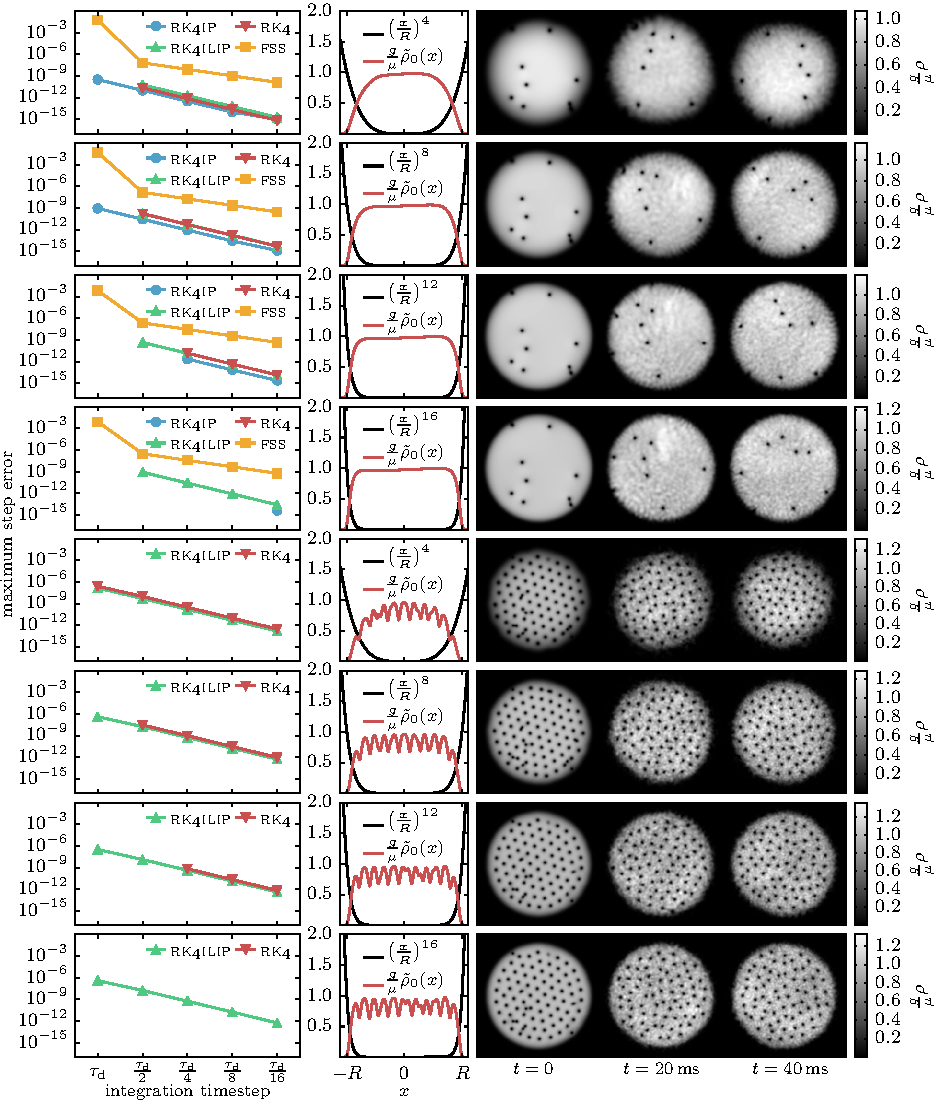
\includegraphics{figures/numerics/rk4ilip_results.pdf}
        \caption{Results of simulations to compare \textsc{rl4ilip} to other timestepping methods.
        Top four rows: Nonrotating frame simulations with four different radial power-law potentials.
        Bottom four rows: Rotating frame simulations with same four potentials.
        Left column: maximum per-step error $\int \abs*{\psi - \tilde\psi}^2\,\dd \vec{r}/\int\abs*{\tilde\psi}^2\,\dd \vec{r}$ of fourth order Runge--Kutta (\textsc{rk4}), its interaction picture variants (\textsc{rk4ip} and \textsc{rk4ilip}) and Fourier split-step (\textsc{fss}) as a function of timestep. Solutions were checked every $100$ timesteps against a comparison solution $\tilde \psi$ computed using half sized steps for \textsc{rk4} methods, and quarter sized steps for \textsc{fss}. Simulations encountering numerical overflow not plotted.
        Centre column: potential (black) and average density $\tilde \rho_0$ of the initial state  (red) over a slice of width $R/5$ in the $y$ direction.
        Right column: Density of solution at initial, intermediate and final times for each configuration simulated (taken from \textsc{rk4ilip} results).
        \textsc{rk4ilip} is the only method usable in rotating frames and not encountering overflow in the steeper traps for the timesteps considered.}
        \label{fig:rk4ilip_results}
    \end{figure}
    \restoregeometry
}

 Here I compare four numerical methods: Fourier split-step (\textsc{fss}), fourth order Runge--Kutta in the interaction picture (\textsc{rk4ip}), ordinary fourth order Runge--Kutta (\textsc{rk4}), and my new method --- fourth order Runge--Kutta in an instananeous local interaction picture (\textsc{rk4ilip}).

 The example chosen is a \textsc{2d} simulation of a turbulent Bose--Einstein condensate, in both a rotating and nonrotating frame. For the nonrotating frame the differential equation simulated was equation \eqref{eq:RK4_ILIP_GPE}, and for the rotating frame the same equation was with an additional two terms added to the Hamiltonian:
\begin{align}
\hat H_\up{rot} + \hat H_\up {comp} &= -\vec \Omega \cdot \hat{\vec L} +\frac12\hbar m^2\Omega^2 r^2\\
                &= i\hbar\Omega \left(x\pdv{y} - y\pdv{x}\right) +\frac12\hbar m^2\Omega^2 r^2.
\end{align}
The addition of the first term transforms the original Hamiltonian into a frame rotating at angular frequency $\Omega$ in the $(x, y)$ plane, and is equivalent to the the Coriolis and centrifugal forces that appear in rotating frames in classical mechanics \cite{Gulshani1978}. The second term is a harmonic potential that exactly compensates for the centrifugal part of this force. In this way the only potential in the rotating frame is the applied trapping potential, and the only effect of the rotating frame is to add the Coriolis force.

 Four trapping potentials were used, all radial power laws with different powers. These examples were chosen to demonstrate the specific situation in which \textsc{rk4ilip} provides a benefit over the other methods for spatial Schr\"odinger-like equations, as discussed above.

The results of $120$ simulation runs are shown in \figref{fig:rk4ilip_results}. Each simulation was of a $\ ^\up{87}$Rb condensate in the $\ket{F=2, m_F=2}$ state, in which the two-body $s$-wave scattering length is $a = 98.98$ Bohr radii \cite{vanKempen2002}. The simulation region was $20\unit{\mu m}$ in the $x$ and $y$ directions, and the Thomas--Fermi radius of the condensate was $R = 9\unit{\mu m}$.  The chemical potential was $\mu = 2\pi\hbar\times 1.91\unit{kHz}$, which is equivalent to a maximum Thomas--Fermi density $\rho_\up{max} = 2.5\E{14}\unit{cm}^{-3}$ and a healing length $\xi = 1.1\unit{\mu m}$. There were $256$ simulation grid points in each spatial dimension, which is $14$ points per healing length.

Four different potentials were used, all of the form $V(r) = \mu \left(r/R\right)^\alpha$ with $\alpha = 4, 8, 12, 16$. For the rotating frame simulations, the rotation frequency was $\Omega = 2\pi \times 148\unit{Hz}$. This is $89\%$ of the effective harmonic trap frequency, defined as the frequency of a harmonic trap that would have the same Thomas--Fermi radius given the same chemical potential.

All ground states were determined using successive over-relaxation (See section [TODO]) with sixth-order finite differences for spatial derivatives. For the nonrotating simulations, convergence was reached with $\upDelta\mu/\mu < 1\E{-13}$, with:
\begin{equation}
\upDelta\mu = \sqrt{\frac{\matrixel{\psi} {(\hat H - \mu)^2}{\psi}}{\braket {\psi}{\psi}}},
\end{equation}
where $\hat H$ is the nonlinear Hamiltonian and $\braket{\vec r}{\psi}$ is the condensate wavefunction, which does not have unit norm. For the rotating frame simulations the ground states converged to $\upDelta\mu/\mu \approx 9\E{-7}, 2\E{-6}, 3\E{-6}$ and $2\E{-6}$ for $\alpha = 16, 12, 8$, and $4$ respectively.

After each ground state was found, it was multiplied by a spatially varying phase factor corresponding to the phase pattern of a number of randomly positioned vortices:
\begin{align}
\psi_\up{vortices}(x, y) = \psi_\up{ground state}(x, y)\prod_{n=1}^N e^{\pm_n i\arctantwo(y - y_n, x - x_n)}
\end{align}
where $\arctantwo$ is the two-argument $\arctan$ function,\footnote{Defined as the principle value of the argument of the complex number $x + iy$: \mbox{$\arctantwo(y, x) = \Arg(x + iy)$.}} $N=30$, $\pm_n$ is a randomly chosen sign, and $(x_n, y_n)$ are vortex positions randomly drawn from a Gaussian distribution centred on $(0,0)$ with standard deviation equal to the Thomas--Fermi radius $R$. The same seed was used for the pseudorandom number generator in each simulation run, and so the vortex positions were identical in each simulation run.

After vortex phase imprinting, the wavefunctions were evolved in imaginary time \cite{chiofalo2000}. For the nonrotating frame simulations, imaginary time evolution was performed for a time interval equal to the chemical potential timescale $\tau_\mu= 2\pi\hbar/\mu$, and for the rotating frame simulations, for $\tau_\mu/10$. This was done to smooth out the condensate density in the vicinity of vortices, producing the correct density profile for vortex cores. However, since imaginary time evolution decreases the energy of the state indiscriminately, it also had the side effect of causing vortices of opposite sign to move closer together and annihilate. This decreased the number of vortices, and is the reason the smoothing step in the rotating frame simulations was cut short to $\tau_\mu/10$, as otherwise all vortices had time to annihilate with one of the lattice vortices. A vortex pair in the process of annihilating is visible in \figref{fig:rk4ilip_results} as a partially filled hole in the initial density profile near the top of the condensate in the $\alpha=4, 12,$ and $16$ rotating frame simulations.\footnote{The initial states for the four different potentials are not identical, so by chance the corresponding vortex in the $\alpha=8$ case was not close enough to a lattice vortex to annihilate.}

The smoothed, vortex imprinted states were then evolved in time for $40\unit{ms}$. For each simulation, five different timesteps were used: $\upDelta t = \tau_\up d, \tau_\up d / 2, \tau_\up d / 4, \tau_\up d / 8, \tau_\up d / 16$, where \mbox{$\tau_\up d = m \upDelta x^2 / \pi\hbar \approx 2.68\unit{\mu s}$} is the dispersion timescale associated with the grid spacing $\upDelta x$, defined as the time taken to move one gridpoint at the phase velocity of the Nyquist mode.

For the nonrotating frame simulations, spatial derivatives for the \textsc{rk4} and \textsc{rk4ilip} methods were determined using the Fourier method [see section TODO]. This was to ensure a fair comparison with the other two methods, which necessarily use Fourier transforms to perform computations pertaining due to the kinetic term.

For the rotating frame simulations, sixth-order finite differences with zero boundary conditions were used instead for the kinetic terms of the \textsc{rk4} and \textsc{rk4ilip} methods, which were the only two methods used for those simulations (due to the other methods being incompatible with the angular momentum operator required for a rotating frame). This choice was fairly arbitrary, but did allow the condensate to be closer to the boundary than is otherwise possible with the periodic boundary conditions imposed by use of the Fourier method for spatial derivatives. This is because the rotating frame Hamiltonian is not periodic in space, and so its discontinuity at the boundary can be a problem if the wavefunction is not sufficiently small there.

As shown in \figref{fig:rk4ilip_results}, all methods tested generally worked well until they didn't work at all, with the per-step error of \textsc{rk4}-based methods being either small and broadly the same as the other \textsc{rk4}-based methods, or growing rapidly to the point of numerical overflow (shown as missing datapoints). The break down of \textsc{fss} was less dramatic, though it too had a clear jump in its per-step error for larger timesteps. Comparing methods therefore came down to mostly whether or not a simulation experienced numerical overflow during the time interval being simulated.

The main result was that \textsc{rk4ilip} and \textsc{fss} remained accurate over the widest range of timesteps and trap steepnesses, with \textsc{rk4} and \textsc{rk4ip} requiring ever smaller timesteps in order to not overflow as the trap steepness increased.

For the rotating frame simulations, which were only amenable to the \textsc{rk4} and \textsc{rk4ilip} methods, the same pattern was observed, with \textsc{rk4} only working at smaller timesteps as the trap steepness was increased, and ultimately diverging for all timesteps tested at the maximum trap steepness. By contrast, \textsc{rk4ilip} remained accurate over the entire range of timesteps at the maximum trap steepness.

\subsection{Discussion}

As mentioned, \textsc{rk4ilip} is mostly useful for continuum quantum mechanics only when there are large spatial differences in the potential, which cannot give rise to equally large kinetic energies\footnote{This is essentially due to such a situation violating the condition we laid out at the beginning of this section --- that the simulation basis must be nearly an eigenbasis of the total Hamiltonian.}. Furthermore, the advantage that \textsc{rk4ilip} has over other methods with that same property is that it is does not require a particular form of Hamiltonian or a particular method of evaluating spatial derivatives. The former means is is applicable in rotating frames or to situations with unusual Hamiltonians, and the latter means is can be used with finite differences or \textsc{fedvr} \cite{schneider2006} and thus is amenable to parallelisation on a cluster computer.

The ability to model large spatial variations in the potential provides only a narrow domain of increased usefulness over other methods. If a large kinetic energy results from the large potential, then the method requires just as small timesteps as any other. And if the large potential is supposed to approximate an an infinite well, then an actual infinite well may be modelled using zero boundary conditions, negating the need for something like \textsc{rk4ilip}. However, when potential wells are steep, but not infinitely steep, here \textsc{rk4ilip} provides a benefit. The only other model that can handle these large potentials---Fourier split-step---has the disadvantage that it cannot deal with arbitrary operators such as those arising from a rotating frame, and is not parallelisable with local data. The benefits of parallelisability are obvious, and the above results demonstrate \textsc{rk4ilip}'s advantage at simulating \textsc{bec}s in tight traps and rotating frames.

For systems with discrete degrees of freedom, \textsc{rk4ilip} may be useful in the case where an approximate diagonalisation of the Hamiltonian is analytically known, and when the Hamiltonian's eigenvalues vary considerably in time (making a single interaction picture insufficient to factor out dynamical phases throughout the entire simulation). In this situation an analytic transformation into the diagonal basis can be performed at each timestep (or the differential equation analytically re-cast in that basis in the first place), and \textsc{rk4ilip} can be used to factor out the time-varying dynamical phase evolution at each timestep. An example may be an atom with a magnetic moment in a time-varying magnetic field which varies over orders of magnitude. The transformation into the spin basis in the direction of the magnetic field can be analytically performed, and if the field varies by orders of magnitude, so do the eigenvalues of the Hamiltonian. Although the eigenvalues in this case and other similar cases can be computed analytically too, unless all time dependence of the Hamiltonian is known in advance of the simulation, it would be difficult to incorporate this into a re-casting of the differential equation in a time-dependent interaction picture. \textsc{rk4ilip} may be useful in these cases to automate this process and evolve the system in the appropriate interaction picture at each timestep.
